\documentclass[tikz,border=10pt]{standalone}
\usetikzlibrary{arrows.meta, positioning, calc, decorations.pathreplacing}
\usepackage{amsmath}
\usepackage{amssymb}

\begin{document}
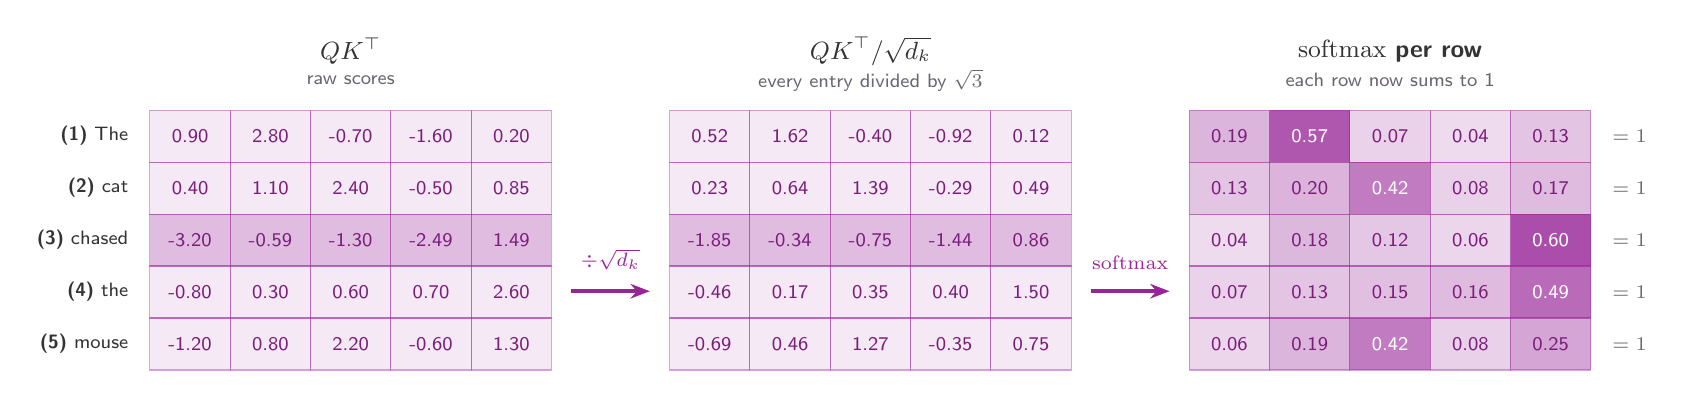
\begin{tikzpicture}[
    every node/.style={font=\sffamily},
]

\definecolor{c1}{HTML}{15173D}
\definecolor{c2}{HTML}{982598}   % scores and weights
\definecolor{c3}{HTML}{E491C9}
\definecolor{c4}{HTML}{F1E9E9}
\definecolor{axiscolor}{HTML}{333333}
\definecolor{labelcolor}{HTML}{6B6472}

\def\cw{1.02}   % cell width
\def\ch{0.66}   % cell height

% ================================================================
% Three 5x5 tables, the same numbers at three stages.
%   raw       top-left (0, 5.4)
%   scaled    top-left (6.6, 5.4)
%   weights   top-left (13.2, 5.4)
% Row 3 is shaded throughout: it is the row whose weights the tutorial
% has been using since the first figure.
% ================================================================

% ---------------------------------------------------------------- raw scores
\begin{scope}[shift={(0,0)}]
  \node[font=\sffamily\small\bfseries, text=axiscolor] at (2.55, 6.15) {$QK^{\top}$};
  \node[font=\sffamily\scriptsize, text=labelcolor] at (2.55, 5.78) {raw scores};

  \foreach \row/\r in {%
      {0.90,2.80,-0.70,-1.60,0.20}/0,
      {0.40,1.10,2.40,-0.50,0.85}/1,
      {-3.20,-0.59,-1.30,-2.49,1.49}/2,
      {-0.80,0.30,0.60,0.70,2.60}/3,
      {-1.20,0.80,2.20,-0.60,1.30}/4} {
    \foreach \v [count=\c from 0] in \row {
      \pgfmathsetmacro{\op}{ifthenelse(\r==2, 0.30, 0.10)}
      \fill[c2, opacity=\op] (\c*\cw, 5.4-\r*\ch-\ch) rectangle ++(\cw, \ch);
      \draw[c2, opacity=0.4, line width=0.4pt]
          (\c*\cw, 5.4-\r*\ch-\ch) rectangle ++(\cw, \ch);
      \node[font=\sffamily\scriptsize, text=c2!80!black]
          at (\c*\cw+0.51, 5.4-\r*\ch-0.33) {\v};
    }
  }
\end{scope}

% ---------------------------------------------------------------- scaled
\begin{scope}[shift={(6.6,0)}]
  \node[font=\sffamily\small\bfseries, text=axiscolor] at (2.55, 6.15)
      {$QK^{\top} / \sqrt{d_k}$};   % inline, so all three titles share a baseline
  \node[font=\sffamily\scriptsize, text=labelcolor] at (2.55, 5.78)
      {every entry divided by $\sqrt{3}$};

  \foreach \row/\r in {%
      {0.52,1.62,-0.40,-0.92,0.12}/0,
      {0.23,0.64,1.39,-0.29,0.49}/1,
      {-1.85,-0.34,-0.75,-1.44,0.86}/2,
      {-0.46,0.17,0.35,0.40,1.50}/3,
      {-0.69,0.46,1.27,-0.35,0.75}/4} {
    \foreach \v [count=\c from 0] in \row {
      \pgfmathsetmacro{\op}{ifthenelse(\r==2, 0.30, 0.10)}
      \fill[c2, opacity=\op] (\c*\cw, 5.4-\r*\ch-\ch) rectangle ++(\cw, \ch);
      \draw[c2, opacity=0.4, line width=0.4pt]
          (\c*\cw, 5.4-\r*\ch-\ch) rectangle ++(\cw, \ch);
      \node[font=\sffamily\scriptsize, text=c2!80!black]
          at (\c*\cw+0.51, 5.4-\r*\ch-0.33) {\v};
    }
  }
\end{scope}

% ---------------------------------------------------------------- weights
\begin{scope}[shift={(13.2,0)}]
  \node[font=\sffamily\small\bfseries, text=axiscolor] at (2.55, 6.15)
      {$\operatorname{softmax}$ per row};
  \node[font=\sffamily\scriptsize, text=labelcolor] at (2.55, 5.78)
      {each row now sums to 1};

  \foreach \row/\r in {%
      {0.19,0.57,0.07,0.04,0.13}/0,
      {0.13,0.20,0.42,0.08,0.17}/1,
      {0.04,0.18,0.12,0.06,0.60}/2,
      {0.07,0.13,0.15,0.16,0.49}/3,
      {0.06,0.19,0.42,0.08,0.25}/4} {
    \foreach \v [count=\c from 0] in \row {
      \pgfmathsetmacro{\op}{0.12 + 1.15*\v}
      \fill[c2, opacity=\op] (\c*\cw, 5.4-\r*\ch-\ch) rectangle ++(\cw, \ch);
      \draw[c2, opacity=0.4, line width=0.4pt]
          (\c*\cw, 5.4-\r*\ch-\ch) rectangle ++(\cw, \ch);
      % dark fills need light numerals
      \pgfmathsetmacro{\vv}{\v}
      \ifdim\vv pt>0.35pt \colorlet{celltext}{white}
      \else \colorlet{celltext}{c2!80!black}\fi
      \node[font=\sffamily\scriptsize, text=celltext]
          at (\c*\cw+0.51, 5.4-\r*\ch-0.33) {\v};
    }
    \node[font=\sffamily\scriptsize, text=labelcolor, anchor=west]
        at (5*\cw+0.15, 5.4-\r*\ch-0.33) {$=1$};
  }
\end{scope}

% ---------------------------------------------------------------- row labels
\foreach \w/\r in {{\textbf{(1)} The}/0, {\textbf{(2)} cat}/1,
                   {\textbf{(3)} chased}/2, {\textbf{(4)} the}/3,
                   {\textbf{(5)} mouse}/4} {
  \node[font=\sffamily\scriptsize, text=axiscolor, anchor=east]
      at (-0.15, 5.4-\r*\ch-0.33) {\w};
}

% ---------------------------------------------------------------- arrows
\draw[-{Stealth[length=7pt]}, line width=1.3pt, c2]
    (5.35, 3.1) -- (6.35, 3.1);
\node[font=\sffamily\scriptsize, text=c2, anchor=south] at (5.85, 3.25)
    {$\div \sqrt{d_k}$};

\draw[-{Stealth[length=7pt]}, line width=1.3pt, c2]
    (11.95, 3.1) -- (12.95, 3.1);
\node[font=\sffamily\scriptsize, text=c2, anchor=south] at (12.45, 3.25)
    {$\operatorname{softmax}$};

\end{tikzpicture}
\end{document}
